\section{Backlog Maintenance}

Managing Backlogs
\newline\newline
Backlogs can be easily maintained. Creating a backlog is the exact same process as creating any other type of model ( use the File menu or the new button on the toolbar). Once you have opened the create window the only things necessary fields on a backlog are the short name and a PO for the backlog.
\newline
Adding a new story to a backlog is easy. Simply select it from the story drop down (optionally give it a priority) and then press add. Prioritised stories will appear at the top of the table, ordered by their priority. Unprioritised stories will appear below them in alphabetical order. To remove a story simply click the delete button (the 'X') on the right hand side of the story table.

\begin{figure}[H]
\centering
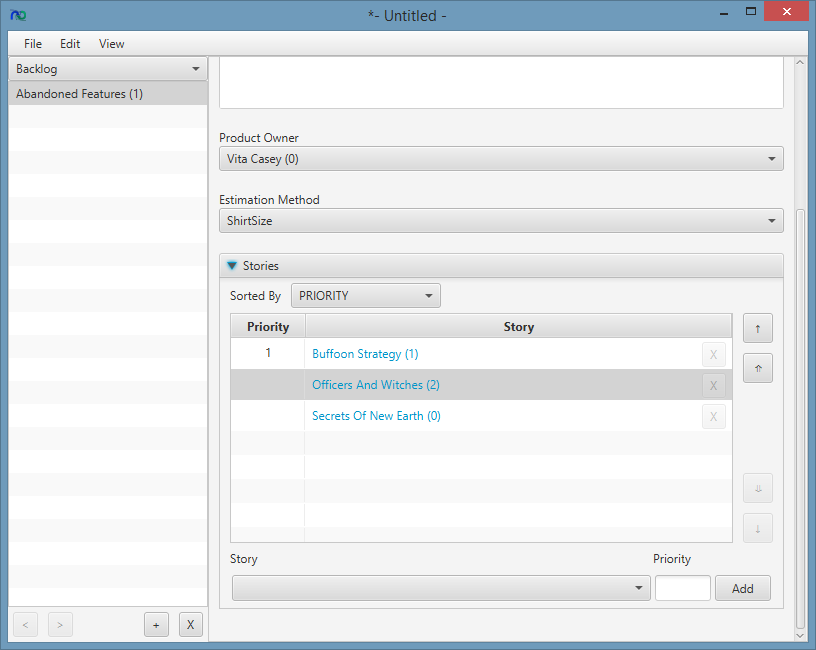
\includegraphics[width=\textwidth]{images/screenshots/backlogs.PNG}
\caption{The Backlogs Edit Pane}
\label{fig:new_project}
\end{figure}

\bigskip
To change the priority of a story simply select it and click on the up and down arrows to the side of the table. The small arrow buttons shift the story one place while the large ones give the story the highest priority or unprioritise it. Alternatively, you may specify the exact priority you wish to change a story to by clicking in the priority column of the story you wish to move, the typing the new priority and pressing enter or else just clicking away.

\begin{figure}[H]
\centering
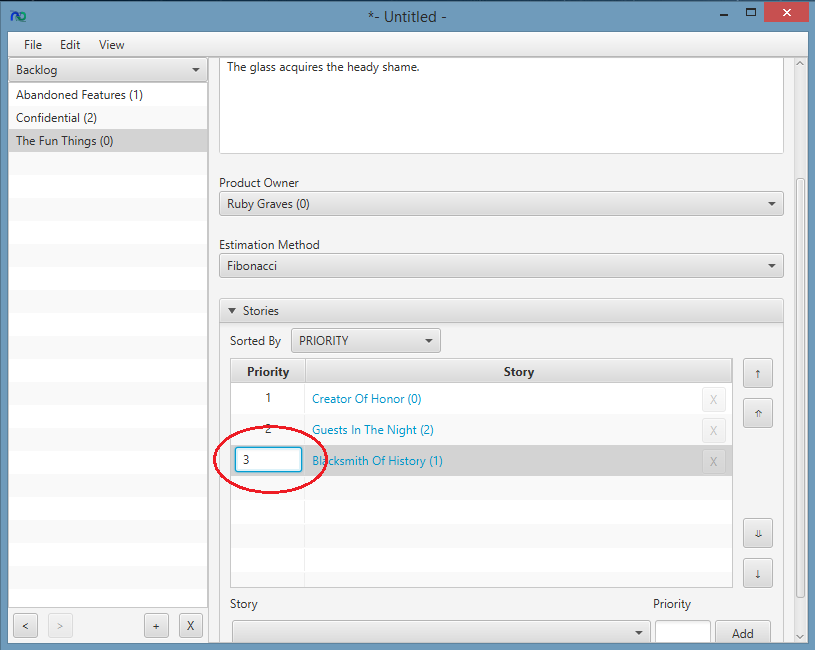
\includegraphics[width=\textwidth]{images/screenshots/editable_priority.PNG}
\caption{Editable Priorities}
\label{fig:new_project}
\end{figure}

\bigskip
If you wish to see a visual representation of the state of the backlog, you may selected the "highlight stories" item in the View menu. This will add a bar to the left of the table of stories that is coloured depending on the readiness state of the story it is beside. It is coloured red when the story depends on another story with a lower priority than itself, green when the story is ready and orange when it is almost ready but still requires an estimation. This feature is turned on by default.

\begin{figure}[H]
\centering
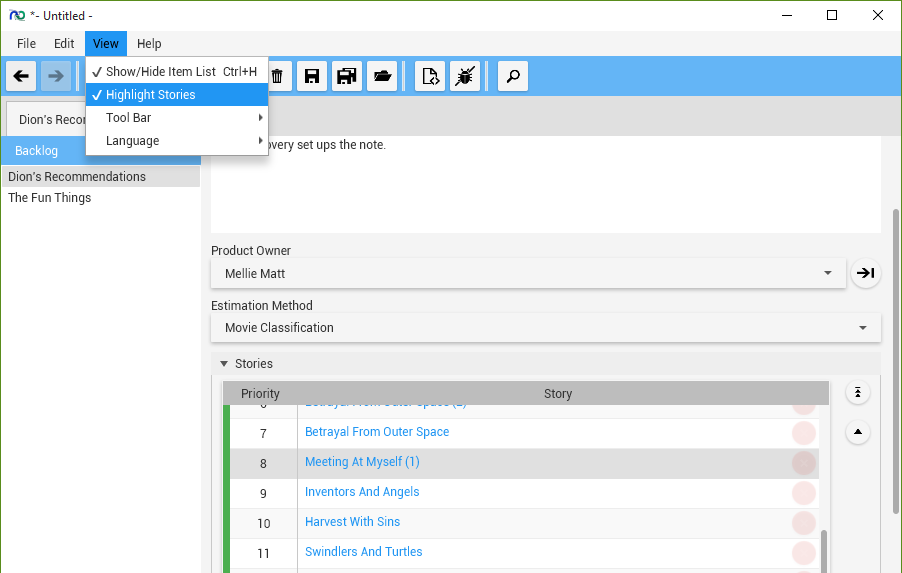
\includegraphics[width=\textwidth]{images/screenshots/story_highlighting.PNG}
\caption{Highlighting Stories}
\label{fig:new_project}
\end{figure}

\bigskip
Estimation Methods
\newline
Estimation methods are systems you use to give a rough approximation of the difficulty of stories within the backlog. The supported types are Fibonacci (1,2,3,5,8,13), ShirtSizes (XS,S,M,L,XL,XXXL) and Movie Ratings (PG,G,M,R16,R18,Banned). You can change this at any time and the program will do its best to convert to the new scale, though it may not be perfect. 

It is also possible to set the estimate as Not Estimated, 0 or Infinite.

\pagebreak
Estimation Workspace
\newline
The estimate workspace is a visual representation of stories in a backlog that have been grouped by common estimates. It enables the user to change the estimate of individual stories by dragging them between different estimate groups.

\begin{figure}[H]
\centering
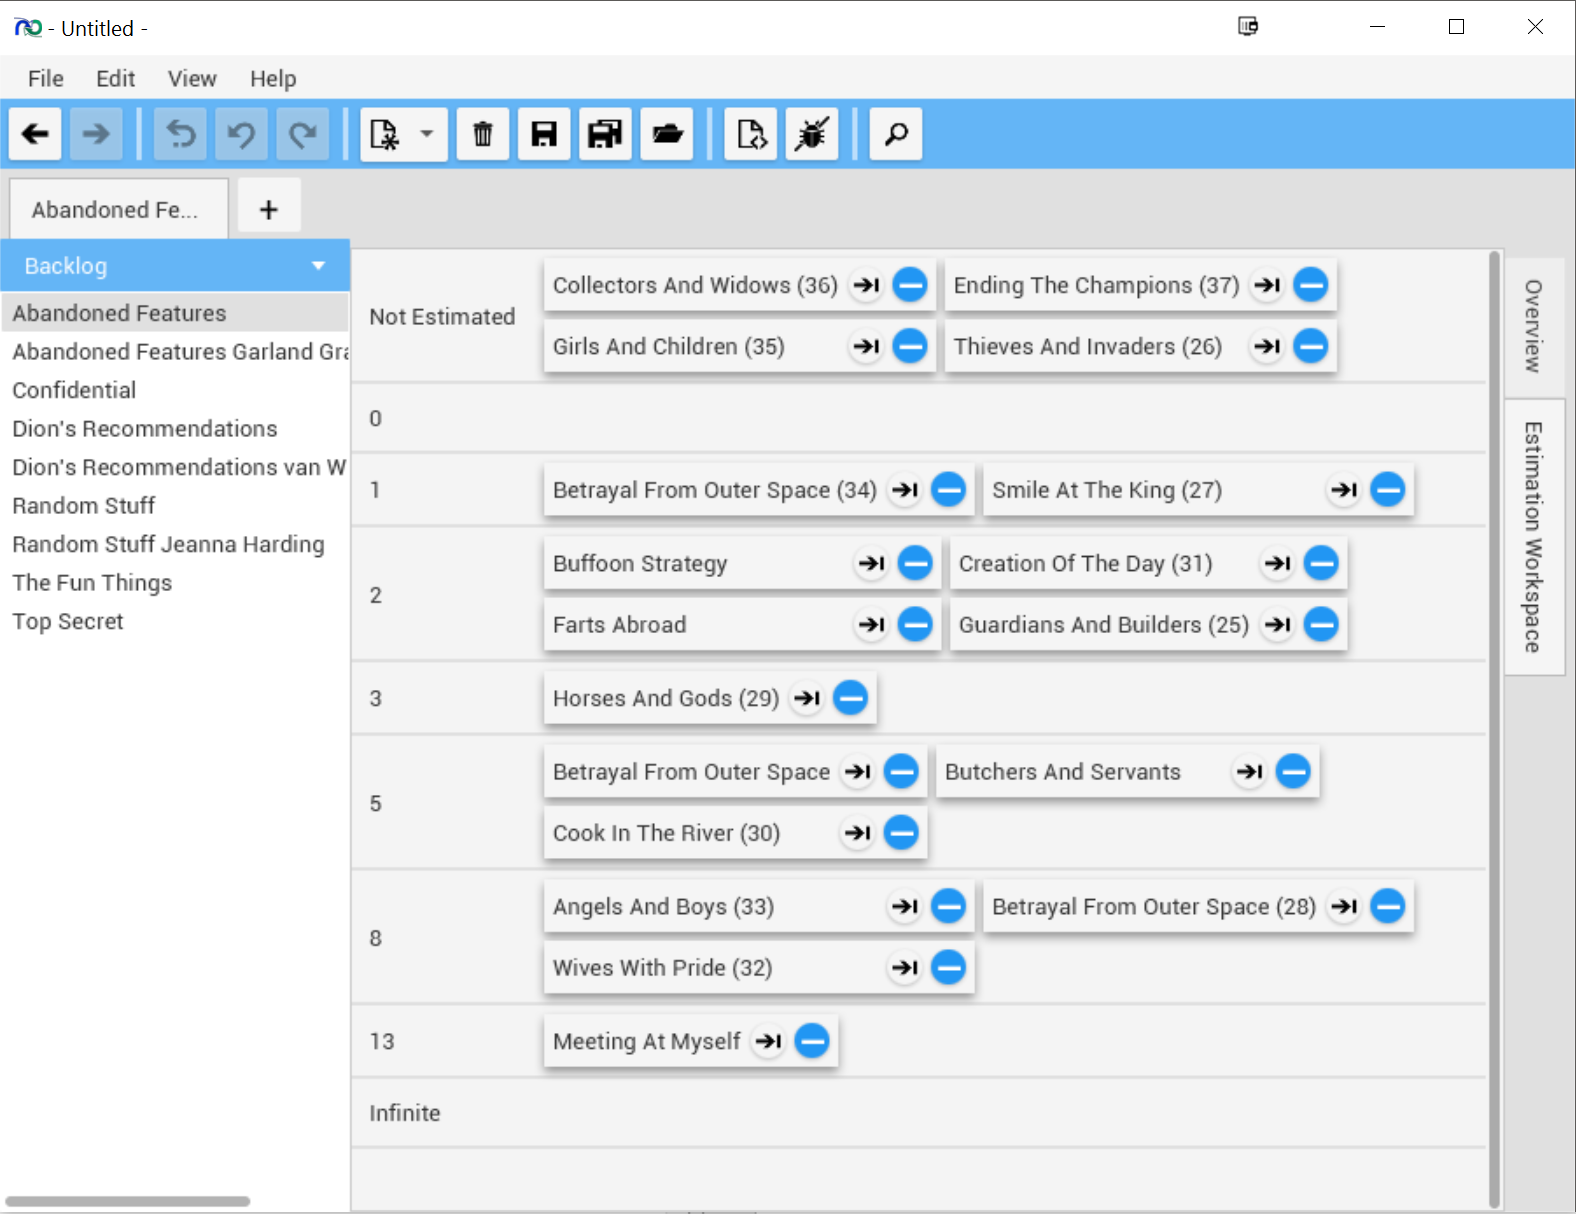
\includegraphics[width=\textwidth]{images/screenshots/estimationWorkspace1.PNG}
\caption{Estimate Workspace}
\label{fig:new_project}
\end{figure}

\pagebreak
Removing and Adding stories to the workspace:
Stories can be added or removed from the workspace via the table of stories in the backlog overview. 
The buttons to do this are shown in the red circles

\begin{figure}[H]
\centering
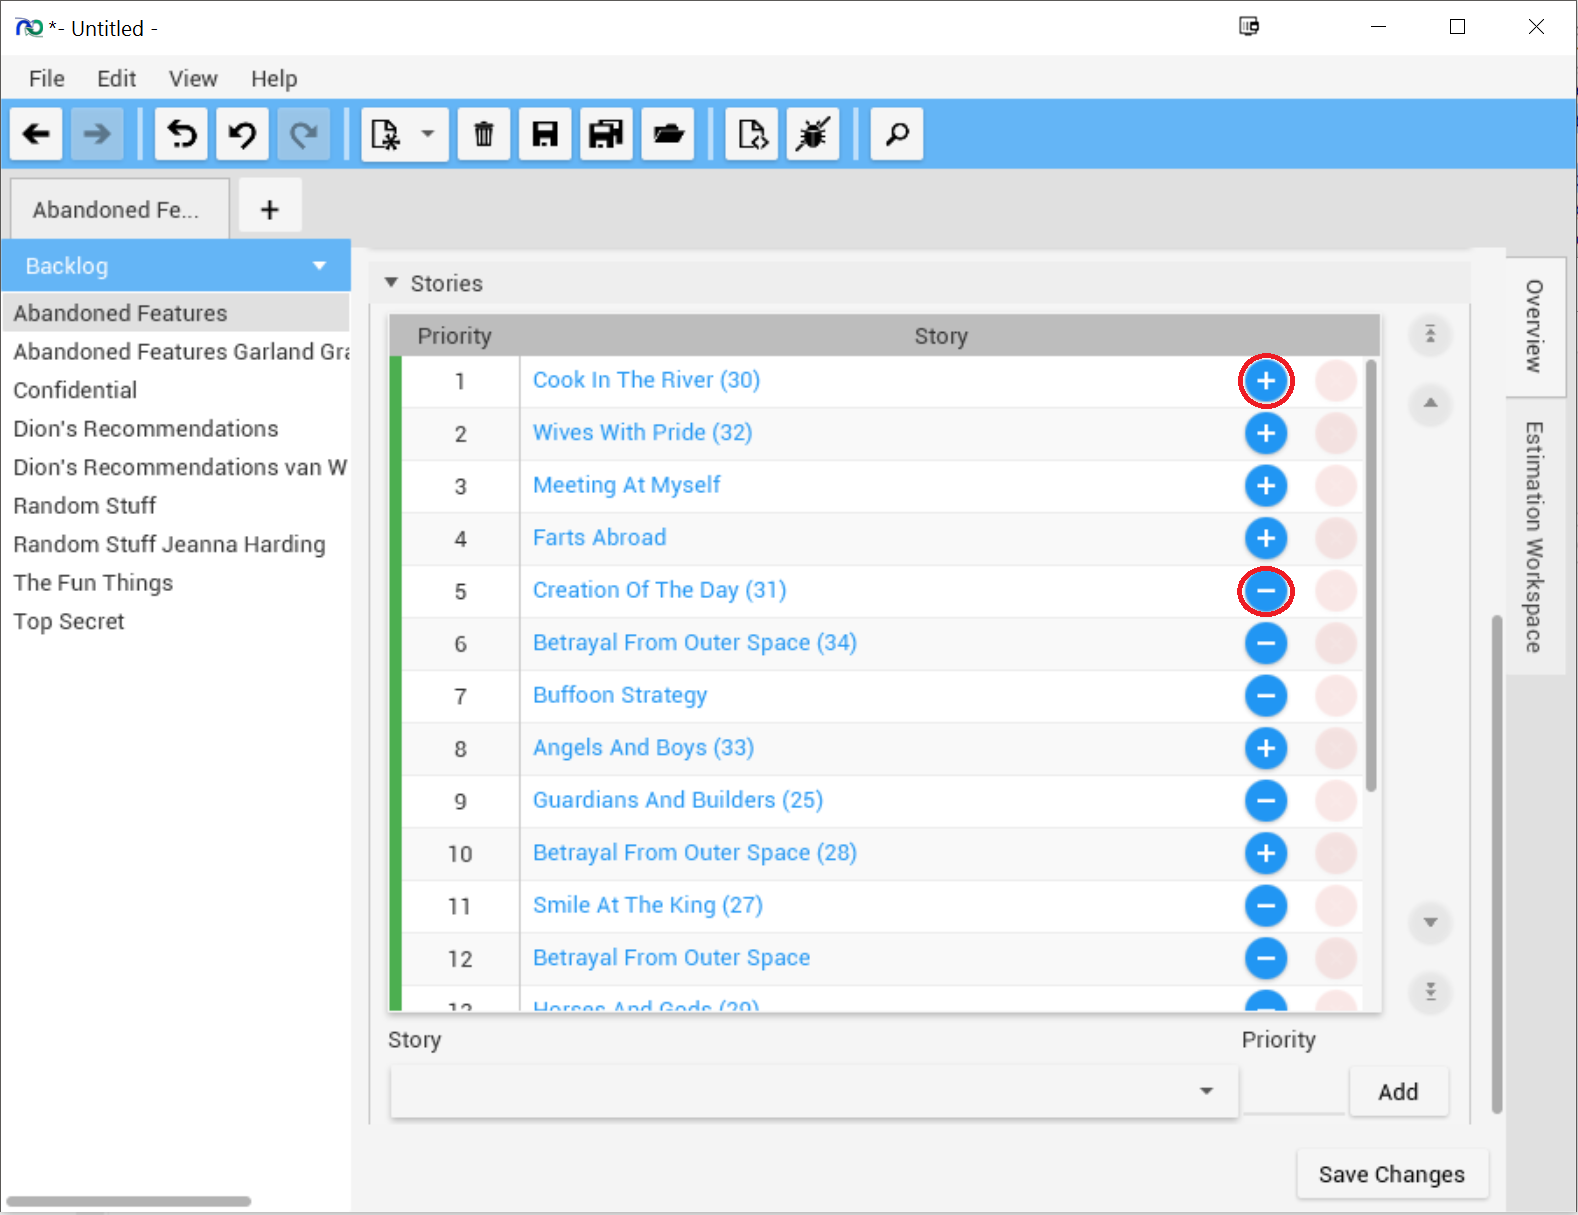
\includegraphics[width=\textwidth]{images/screenshots/estimationWorkspace2.PNG}
\caption{Adding and removing stories from the estimation workspace}
\label{fig:new_project}
\end{figure}

\pagebreak
You can also remove stories directly from the workspace by pressing the button shown in the red circle below.

\begin{figure}[H]
\centering
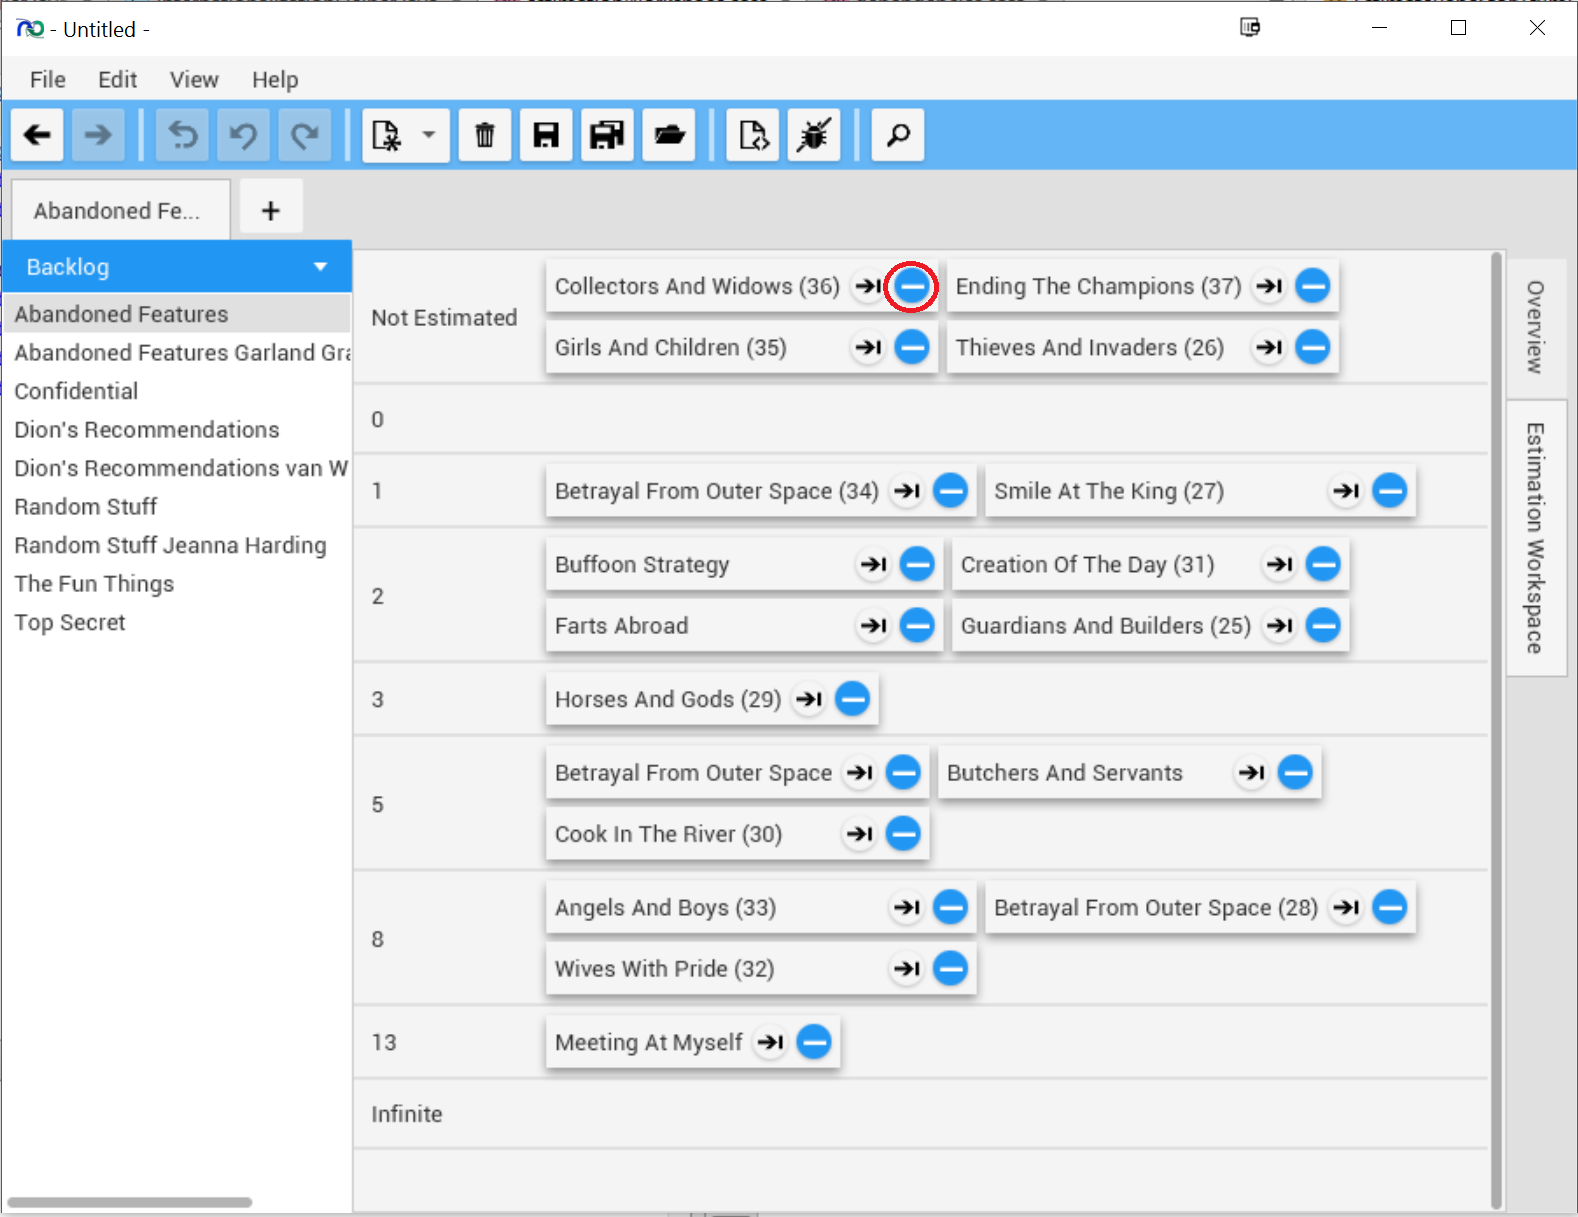
\includegraphics[width=\textwidth]{images/screenshots/estimationWorkspace3.PNG}
\caption{Removing stories from within the estimation workspace}
\label{fig:new_project}
\end{figure}

\pagebreak
Navigating to stories from within the workspace:\newline
A story can be navigated to from within the workspace be selecting the button circled in red below.

\begin{figure}[H]
\centering
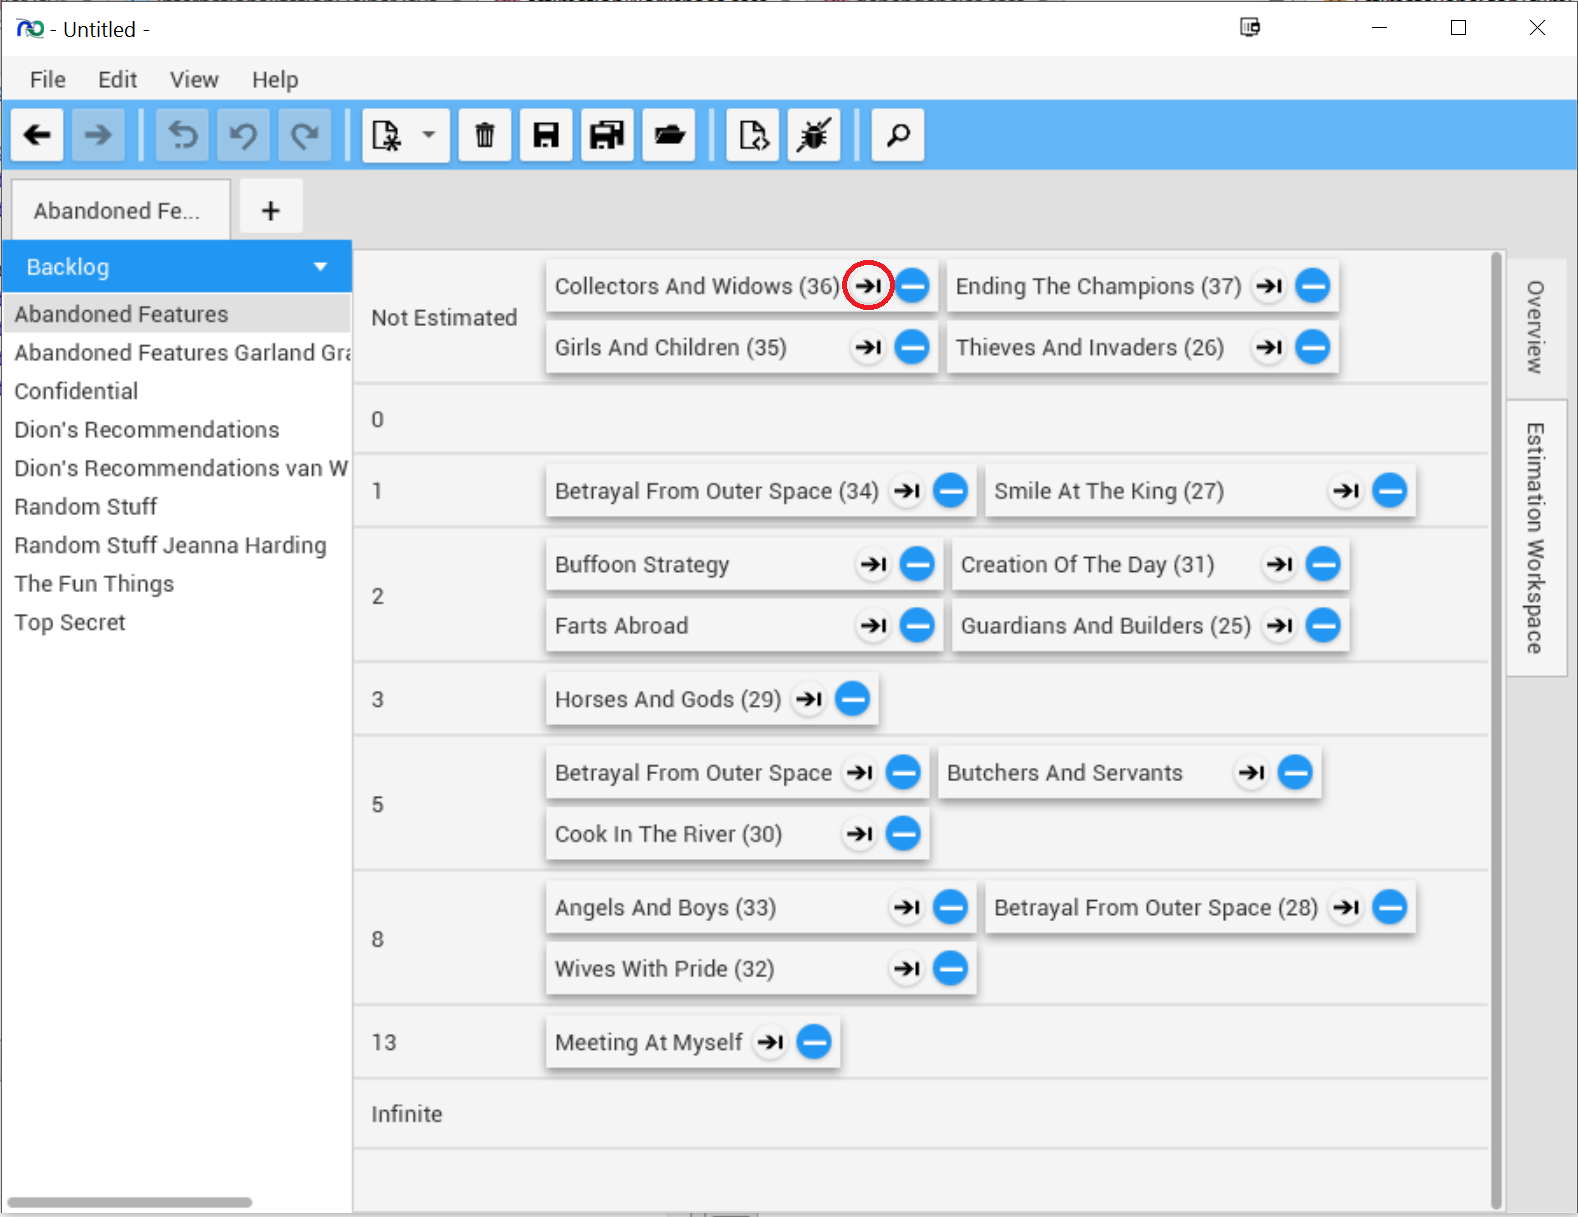
\includegraphics[width=\textwidth]{images/screenshots/estimationWorkspace4.PNG}
\caption{Navigate to a story from within the estimation workspace}
\label{fig:new_project}
\end{figure}






